\documentclass{article}
\usepackage[utf8]{inputenc}
\usepackage[margin=1in]{geometry}
\usepackage[T1]{fontenc}
\usepackage{graphicx}
\usepackage{tikz}
\usetikzlibrary{positioning}
\usetikzlibrary{shadows,trees}
\usepackage{enumitem}
\usepackage{pdfpages}

\begin{document}

\begin{titlepage} % Suppresses displaying the page number on the title page and the subsequent page counts as page 1
	\newcommand{\HRule}{\rule{\linewidth}{0.5mm}} % Defines a new command for horizontal lines, change thickness here
	
	\center % Centre everything on the page
	
	%------------------------------------------------
	%	Headings
	%------------------------------------------------
	
	\textsc{\LARGE University of Manitoba}\\[1.5cm] % Main heading such as the name of your university/college
	
	\begin{figure}
	    \centering
	    
\includegraphics[width=1in]{uofmlogo.png}
	    \label{fig:uofm}
	\end{figure}
	
	\textsc{\Large COMP 3020}\\[0.5cm] % Major heading such as course name
	
	\textsc{\large Human Computer Interaction I}\\[0.5cm] % Minor heading such as course title
	
	%------------------------------------------------
	%	Title
	%------------------------------------------------
	
	\HRule\\[0.4cm]
	
	{\huge\bfseries Group 20: Milestone 2}\\[0.4cm] % Title of your document
	
	\HRule\\[1.5cm]
	
	%------------------------------------------------
	%	Author(s)
	%------------------------------------------------
	
	\begin{minipage}{0.4\textwidth}
		\begin{flushleft}
			\large
			\textit{Authors}\\
			Skylar \textsc{Greenslade}, 7795032\\
			Charle \textsc{Amao}, 7763900\\% Your name
			Sanjay \textsc{Abraham}, 7793952\\
			Seunghwan \textsc{Youn}, 7846681
			
		\end{flushleft}
	\end{minipage}
	~
	\begin{minipage}{0.4\textwidth}
		\begin{flushright}
			\large
			\textit{Professor}\\
			Dr. Jim \textsc{Young} % Supervisor's name
		\end{flushright}
	\end{minipage}

	
	\vfill\vfill\vfill % Position the date 3/4 down the remaining page
	
	{\large\today} % Date, change the \today to a set date if you want to be precise

	\vfill % Push the date up 1/4 of the remaining page
	
\end{titlepage}
\newpage

%~~~~~~~~~~~~~~~ TOC ~~~~~~~~~~~~~~~~~~~
\pagenumbering{gobble}
\tableofcontents
\newpage
%~~~~~~~~~~~~~~~~~~~~~~~~~~~~~~~~~~~~~~~~
\pagenumbering{arabic}

\section{Group Brainstorming}
%Summary of brainstorming process
To come up with good ideas for our project design, our group got together to brainstorm by sketching many ideas. Before meeting, our group reviewed the requirements as previously defined in Milestone 1. This was to encourage us to consider the requirements as each group member prepared to brainstorm.
\newline
\newline
During the brainstorming session, our group sat around a table and drew sketches of any ideas that came to mind. After each group member had drawn their ideas, we took turns sharing the ideas behind each sketch that was drawn. This cycle of drawing and sharing was repeated several times, allowing the group to iterate and be inspired by the ideas shared by the other members, while ensuring that new ideas were included in each sketch. The process was repeated until the group felt that a fairly exhaustive range of ideas had been produced, for each aspect of the potential interface.
\newline
\newline
The functional and data requirements did not have a strong impact on the brainstorming session, as they could all easily be fulfilled without much interface design. All ideas that focused on the entire interface included a visualization of the user's schedule and class information, which assumed some method of meeting the requirements of generating schedule options, allowing the user to experiment, providing a finalized schedule, and more. The usability requirements more significantly guided the brainstorming. When designing a visualization of the schedule, many different ideas were presented, ranging from traditional calendar formats, to more abstract representations of days being lines of different thicknesses to represent filled time slots and conflicts. Many ideas for resolving conflicts were presented. Selecting from generated possibilities, arranging the personal priorities and preferences of classes, or directly selecting a choice between two conflicting classes were some ideas the group generated. Showing class descriptions was one requirement that also had a lot of distinct design ideas. Scroll-able windows with very in-depth information was one idea, contrasted by another idea of showing each class on a card which outlined the class in brief. 
\newline
\newline
Coming up with a learnable design was important, and led to many different ideas. Using conventions such as versatile search bars or drag and drop interfaces was suggested. Minimalist designs and real-time scheduling were prevalent aspects of many ideas, but manifested in distinct ways. Simplifying representations of classes and showing more information on mouse-over was one suggested way to accomplish this. Having consistent windows in the design which contained different types of information was another. Cards containing all class information could keep the correlation between a class and its time slot strong, but a more abstract representation could allow for showing the important aspects of the schedule clearly, without requiring the user to interpret and filter out as much information.
\newline
\newline
Having a large amount of distinct ideas was an important part of coming up with a good design. This allowed for comparing each potential design to many other options, to either ensure that it indeed was a good option, or that there is more preferable deign choice to be made. Brainstorming as a group helped to generate ideas which may not have been considered otherwise, and coming up with so many designs meant that unique options were explored, and a wealth of options were presented.



\section{Idea Polishing}
From the ideas generated during the brainstorming session, three ideas which the group considered to be among the best were selected. These ideas have been sketched in greater detail and explained in this section.
%One paragraph each for describing the idea, and justifying why the sketch is appropriate (per subsection)
%One page per sketch
\subsection{Idea 1: Class-priority}%Rename these?
\subsubsection{Description}
The first idea is centered around a student-specified class-priority list for creating class schedules for a term. To start the schedule generating process, the student will use the search bar to search for classes they find interesting or need to take for their degree. Students can then add these courses to a priority-ranking system that our new website will use to generate possible class schedules. The student can then sift through the generated class schedules and pick the one they like the most. The student may even modify their chosen class schedule or modify the class-priority list in order for the website to generate new schedules. The website will generate schedules based on a simple algorithm that will be determined for the hi-fidelity prototype should the team choose to incorporate this design. For this idea, the website will use a time-horizontal timetable to display the class schedule(s) to students. This allows the timetable to take up less space to display class schedules and allows course information to be displayed beside the timetables; this means there can be more relevant information that is displayed to the user. 

\begin{figure}[!h]
\centering
\caption{Sketch of idea 1.}
\includegraphics[width=14cm]{"Sketch_2_COMP_3020".png}
\end{figure}

\subsubsection{Justification}
The sketch is appropriate because it portrays why the class-priority idea fulfills the user requirements specified in Milestone 1. The sketch shows a visual mock-up of the class-priority system that the website uses to generate schedules. This feature of the website fulfills functional requirements 1 and 2 from Milestone 1; namely that the app or website will generate schedules based on user input and will allow users to experiment with different schedules. The sketch also shows that course information can be viewed using a pane displayed below the timetable. This satisfies the functionality requirements 3 and 4: providing the user with a list of approved courses and informing the user of the necessary prerequisites for the course. The sketch also shows a mock-up of the schedule timetable that shows user-specified "unavailable" time-slots. These time-slots are times in which users will not desire to have classes in (e.g. due to a shift at work). This satisfies the usability requirements such as 1 and 2 in that it implements a visualization method for the user's schedule that fits their mental model and enables the user to visualize and resolve scheduling conflicts with little effort.

\subsection{Idea 2: Course Work-space and Experimental Timetable}%Rename?
\subsubsection{Description}
The second idea utilizes a more user-involved scheduling philosophy than the class-priority idea. Whereas the class-priority automatically generates possible class schedules based on a user-specified priority, the second idea focuses on aiding the user in generating their own ideal schedules by providing them with tools such as a course work-space and an experimental timetable. The course work-space feature allows the user to "store" courses that the user is thinking of taking but is not yet sure of where it fits in the schedule. The experimental timetable mainly refers to a schedule timetable that allows the user to visually experiment with different classes to eventually arrive at the user's ideal schedule, as opposed to Aurora where the user can not experiment using the website at all and will instead need to rely on external tools such as a piece of paper. Once the user is satisfied, they may then formally register for the courses at the press of a button. Any course in the work-space that the user does not have prerequisites or will conflict with the current timetable schedule will be shaded red. This allows the user to easily see potential conflicts and issues.

\begin{figure}[!h]
\centering
\caption{Sketch of idea 2.}
\includegraphics[width=14cm]{"Sketch_1_COMP_3020".png}
\end{figure}

\subsubsection{Justification}
The sketch for idea 2 shows that this idea satisfies most of the usability requirements outlined in Milestone 1. Like idea 1, by utilizing a timetable to display the schedules, the sketch shows that the website enables the user to easily visualize their schedules. The sketch also shows what happens when it is not possible to add any course from the work-space to the active schedule; namely the course would be colored red if the student did not have the necessary prerequisites or if the course would conflict with the active schedule. This feature satisfies usability requirement 2 from Milestone 1, as it allows the user to visualize and resolve scheduling conflicts with little mental effort.

\subsection{Idea 3: Course Filter and Suggestions}%Rename?
\subsubsection{Description}
The third idea combines certain aspects of ideas 1 and 2, namely the "unavailable" slot feature from idea 1 and the experimental timetable from idea 2, along with new features; one such feature is the filters pane. The filters pane allows the student to filter results when they are searching for possible courses to take. For example, if the student just wants to search for courses with no lab component, they can simply add the filter 'No lab component' to filter out their search results. This idea also introduces the suggestions pane feature. This feature suggests courses that the website thinks the user may want to take. This feature will utilize an algorithm that will be based on the variables such as the student's major, courses taken so far, current active schedule, and active filters. The website based on this idea will also allow the students save multiple schedules per term to allow the student to compare different possible schedules and select the best one.

\begin{figure}[!h]
\centering
\caption{Sketch of idea 3.}
\includegraphics[width=14cm]{"Sketch_3_COMP_3020".png}
\end{figure}

\subsubsection{Justification}
Like in sketch 1, by showing the "unavailable" time slot feature, the sketch shows that this idea helps satisfy the usability goals 1 and 2 from Milestone 1. As described earlier, the sketch also shows what the filters and suggestions pane might look like in the final design. This fulfills the usability requirement of the website being easy to learn for students, as most students understand how filters and suggestions are used.


%~~~~~~~~~~~~~~~~~~~~~~~~~~~~~~~~~~~~~~~~~~~~~~~~~~~~~~~~~~~~~~~~~~~~~~~~~~~~~~~~~~~~~~~~
\newpage
\section{Hierarchical Task Graphs}
Three major tasks were selected in relation to the goals of the design. These tasks are (1) adding classes to a short list to be considered, (2) researching individual courses in depth to become more familiar with the options, and (3) resolving conflicts that arise when two or more classes share the same time slot. Each task was analyzed and a hierarchy of steps was created for each. These are represented in the following task graphs.
\subsection{Adding Classes}
\vspace{1ex}

    \begin{tikzpicture}[
      every node/.style = {draw, rounded corners=3pt, semithick, drop shadow},
            ROOT/.style = {top color=green!60!blue, bottom color=blue!60!green,
                             inner sep=2mm, text=white, font=\bfseries},
              L1/.style = {fill=blue!20},
              L2/.style = {fill=orange!30},
              L3/.style = {fill=green!30, grow=down, anchor=west, 
              %L3/.style = {fill=green!30, grow=down, xshift=3em, anchor=west, 
      edge from parent path={(\tikzparentnode.south west) |- (\tikzchildnode.west)}},
edge from parent/.style = {draw, thick},
             LD/.style = {level distance=#1ex},
             LD1/.style = {level distance=6ex},
             LD2/.style = {level distance=12ex},
             LD3/.style = {level distance=18ex},
         level 1/.style = {sibling distance=60mm}
                        ]
    % Parents
\node[ROOT] {Add Class}
    [edge from parent fork down]
    child{node[L2, below = 0f ROOT, text width=5cm] {1. Check degree flow chart for what classes need to be taken}
            }
    child{node[L2, below = 0f ROOT, text width=5cm] {2. Search Courses}
      child[L3,LD1]  {node(b1)[L3, xshift=0.5em, below = of parent, yshift=1.5em, text width = 12em]    {2.1 Search by title}}
      child[L3,LD2]  {node(b2)[L3, below = of b1, text width = 12em]   {2.2 Search by course number}}
      child[L3,LD2]  {node(b3)[L3, below = of b2, text width = 12em]   {2.3 Search by professor name}}
            }
    child {node[L2, below = 0f ROOT, text width=5cm] {3. Choose a Class and add it to the list}
      child[L3,LD1] {node(c1)[L3, xshift=0.5em, below = of parent, yshift=1.5em, text width = 12em]    {3.1 Choose course}}
      child[L3,LD2] {node(c2)[L3, below = of c1, text width = 12em]   {3.2 Choose section}}  
      child[L3,LD3]  {node(c3)[L3, below = of c2, text width = 12em]   {3.3 Choose lab (if there is a lab required}}
            };
\end{tikzpicture}

\subsubsection{Plan 0}
     Do steps 1-2-3 to find what courses need to be taken and add them to a shortlist.
    
\subsubsection{Plan 2}
    Use any sub-task 2.1, 2.2, or 2.3 to find a course.

\subsubsection{Plan 3}
    Do sub-task 3.2 and 3.3 if more than one section exists, and if a lab section is required.


%~~~~~~~~~~~~~~~~~~~~~~~~~~~~~~~~~~~~~~~~~~~~~~~~~~~~~~~~~~~~~~~~~~~~~~~~~~~~~~~~~~~~~~~~



\subsection{Researching Individual Courses}
\vspace{1ex}

    \begin{tikzpicture}[
      every node/.style = {draw, rounded corners=3pt, semithick, drop shadow},
            ROOT/.style = {top color=green!60!blue, bottom color=blue!60!green,
                             inner sep=2mm, text=white, font=\bfseries},
              L1/.style = {fill=blue!20},
              L2/.style = {fill=orange!30},
              L3/.style = {fill=green!30, grow=down, anchor=west, 
              %L3/.style = {fill=green!30, grow=down, xshift=3em, anchor=west, 
      edge from parent path={(\tikzparentnode.south west) |- (\tikzchildnode.west)}},
edge from parent/.style = {draw, thick},
             LD/.style = {level distance=#1ex},
             LD1/.style = {level distance=6ex},
             LD2/.style = {level distance=12ex},
             LD3/.style = {level distance=18ex},
         level 1/.style = {sibling distance=45mm}
                        ]
    % Parents
\node[ROOT] {Research Individual Course}
    [edge from parent fork down]
    child{node[L2, below = 0f ROOT, text width=3.5cm] {1. Read description of selected course to ensure it is in line with the user's requirements}
            }
    child{node[L2, below = 0f ROOT, text width=3.5cm] {2. Identify prerequisites associated with the course being selected}
            }
    child {node[L2, below = 0f ROOT, text width=3.5cm] {3. Analyze the available sections for the selected course}
      child[L3,LD1] {node(c1)[L3, xshift=0.5em, below = of parent, yshift=1.5em, text width = 10em]    {3.1 Read through the various time slots in which the course is available}}
      child[L3,LD2] {node(c2)[L3, below = of c1, text width = 10em]   {3.2 Read through the availability of seats in the various sections}}  
      child[L3,LD3]  {node(c3)[L3, below = of c2, text width = 10em]   {3.3 Read through the section's instructor information such as education, research interests, other courses taught, and general ratings}}
            }
    child {node[L2, below = 0f ROOT, text width=3.5cm] {4. Read comments and reviews}
      child[L3,LD1] {node(d1)[L3, xshift=0.5em, below = of parent, yshift=1.5em, text width = 10em]    {4.1 Read comments from past students regarding the instructor}}
      child[L3,LD2] {node(d2)[L3, below = of d1, text width = 10em]    {4.2 Read comments from past students regarding the course}}
            };
\end{tikzpicture}

\subsubsection{Plan 0}
    If the user has no background information on the course or instructor, do steps 1-2-3-4.
\subsubsection{Plan 3}
    If the user has background information on the course and its prerequisites, and knows what courses they will need to take for their degree, do steps 3-4.
    


%~~~~~~~~~~~~~~~~~~~~~~~~~~~~~~~~~~~~~~~~~~~~~~~~~~~~~~~~~~~~~~~~~~~~~~~~~~~~~~~~~~~~~~~~




\subsection{Resolving Schedule Conflicts}
\vspace{1ex}


    \begin{tikzpicture}[
      every node/.style = {draw, rounded corners=3pt, semithick, drop shadow},
            ROOT/.style = {top color=green!60!blue, bottom color=blue!60!green,
                             inner sep=2mm, text=white, font=\bfseries},
              L1/.style = {fill=blue!20},
              L2/.style = {fill=orange!30},
              L3/.style = {fill=green!30, grow=down, anchor=west, 
              %L3/.style = {fill=green!30, grow=down, xshift=3em, anchor=west, 
      edge from parent path={(\tikzparentnode.south west) |- (\tikzchildnode.west)}},
edge from parent/.style = {draw, thick},
             LD/.style = {level distance=#1ex},
             LD1/.style = {level distance=6ex},
             LD2/.style = {level distance=12ex},
             LD3/.style = {level distance=18ex},
         level 1/.style = {sibling distance=60mm}
                        ]
    % Parents
\node[ROOT] {Resolve most significant conflict}
    [edge from parent fork down]
    child{node[L2, below = 0f ROOT, text width=5cm] {1. Determine most important class between conflicting classes}
      child[L3,LD1]   {node(a1)[L3, xshift=0.5em, below = of parent, yshift=1.5em, text width = 12em]   {1.1 Compare classes' priority for program enrolled in}}
      child[L3,LD2]  {node(a2)[L3, below = of a1, text width = 12em]   {1.2 Compare other possibilities for each class}}
      child[L3,LD3]   {node(a3)[L3, below = of a2, text width = 12em]   {1.3 Compare other preferences such as location, professor, et cetera}}
      child[L3,LD3]   {node(a4)[fill=green!30, below = of a3, text width = 12em]   {1.4 Select the class that is most important to be taken, or preferred}}
            }
    child{node[L2, below = 0f ROOT, text width=5cm] {2. Update schedule planner for the time slot of the conflict}
      child[L3,LD1]  {node(b1)[L3, xshift=0.5em, below = of parent, yshift=1.5em, text width = 12em]    {2.1 Record the class that is chosen for the time slot}}
      child[L3,LD2]  {node(b2)[L3, below = of b1, text width = 12em]   {2.2 Remove other class(es) from the time slot}}
            }
    child {node[L2, below = 0f ROOT, text width=5cm] {3. Ensure less important class(es) priority is compared to other classes}
      child[L3,LD1] {node(c1)[L3, xshift=0.5em, below = of parent, yshift=1.5em, text width = 12em]    {3.1 Check unselected class(es)' priority against other classes that are chosen}}
      child[L3,LD2] {node(c2)[L3, below = of c1, text width = 12em]   {3.2 Consider unselected class(es) possible times, and compare them to current schedule}}  
      child[L3,LD3]  {node(c3)[L3, below = of c2, text width = 12em]   {3.3 Resolve new conflicts among aforementioned classes}}
            };
\end{tikzpicture}
\newline
\newline
\subsubsection{Plan 0}
    Do steps 1, 2, 3 in that order.
\subsubsection{Plan 1}
    If more important class is undetermined, do steps 1.1, 1.2, and 1.3 in order until priority is determined. then do step 1.4.
\subsubsection{Plan 2}
    To update the current schedule, do steps 2.1 and 2.2, in that order.
\subsubsection{Plan 3}
    If less important class(es) are not easily addressed, do steps 3.1, 3.2, and 3.3 in that order. Continue to resolve conflicts among the remaining courses using this task graph until all conflicts are resolved.
%~~~~~~~~~~~~~~~~~~~~~~~~~~~~~~~~~~~~~~~~~~~~~~~~~~~~~~~~~~~~~~~~~~~~~~~~~~~~~~~~~~~~~

\section{Low - Fidelity Prototypes}
To put the ideas to the test, low-fidelity prototypes were created. These prototypes allowed our group to quickly create mock-ups of potential interfaces and features, and gain a better understanding of how they might actually function and be used. Creating these prototypes helped to provide insight into limitations and possibilities of each design element, and allowed the designs to be shown to research participants. The designs focused on the major tasks outlined in section 3 of this report, and also afforded the opportunity to experiment with some contrasting design choices our group considered.

%Summaries of scopes of prototypes, and instructions to understand/use each prototype
\subsection{Paper Prototype 1}%Rename?
The first paper prototype our group created focused on the major tasks adding classes, and resolving conflicts. The prototype is comprised of three sections. The left column contained a search bar for finding classes, and a work space in which classes would be listed and prioritized. on the top to the right of the column was an area where detailed class information would be displayed. The remaining space showed a weekly schedule, with the y-axis listing days of the week, and the x-axis dividing each day into time slots from 8:30am to 5:30pm.
\begin{figure}[h]
	    \centering
	    \caption{Model of Paper Prototype 1}
	    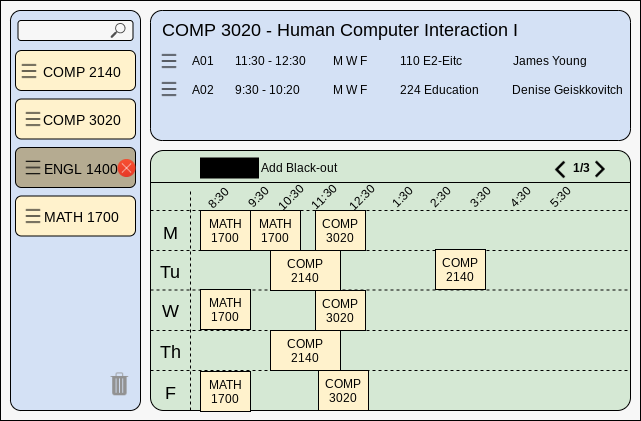
\includegraphics[width=15cm]{paperprototype1.png}
	\end{figure}
	
\noindent
The search bar was designed to be intuitive, and to allow for many ways to search for classes, including typing the course code and number, professor name, course name, or other relevant information. A drop down menu would appear in real time and display suggestions for classes, based on the input. For the purposes of this prototype, predetermined lists of "COMP" courses were included to portray the capabilities and options. Upon mousing over the options shown, the section for more details would become populated with class information. It would display the course name and code at the top, and list all the sections with relevant information in rows beneath the title. Clicking on a course would add it to the work space.
\newline
\newline
Within the work space column, classes would be represented by a card which contained the course code and number for the class. Selecting a card would show the additional details in the upper right portion of the screen again. Classes could be dragged into any order, with higher priority classes at the top of the list, and lower priority at the bottom. Classes could also be removed from the list by dragging them to a trash can icon at the bottom of the column.
\newline
\newline
Upon adding classes to the work space, the schedule would automatically be populated with blocks representing the classes selected. If more than one schedule was possible, the user would be able to view additional schedules by clicking on arrows beside a page count that showed which schedule they were viewing, out of how many were available. As classes were added to the work space, if there was a scheduling conflict that caused one class to be unable to be included, the card representing that class would be shaded, and include an "X" icon to indicate this. The user could then mouse over the card, when a tool-tip would explain what higher priority class prevented the class from being included. The user could then respond by re-prioritizing their list, or allowing the program to automatically schedule a lower priority class that did fit the timetable.
\newline
\newline
In addition to being able to prioritize each class against the others, the individual sections of each class could be prioritized in two different ways. First of all, within the detailed information, if a certain section of the class or lab was listed higher than the others, it would be higher priority for the program to schedule. The user would be able to rearrange these within the detailed information field to their order of preference. Secondly, each individual section of classes or labs could be dragged out of the detailed information section, and placed in the work space. This allows for more advanced prioritizing beyond the comparison of two classes, to being able to prioritize specific lecture or lab sections entirely comprehensively.
\newline
\newline
The final feature included in this paper prototype was a "black-out" function. Above the graphical schedule was a labelled black box which could be dragged onto the schedule. Anywhere one of these boxes was placed would not be considered an available time slot by the schedule planning software. These boxes could be expanded or condensed to restrict times in the schedule as specifically as desired by the user.  Using this and the other features of the prototype would allow for our group to collect feedback on proposed methods of adding classes to a planner easily, and experimenting with resolving conflicts in an efficient and effective way.



\subsection{Paper Prototype 2}%Rename?
%Summary of scope of prototype, and instructions to understand/use the prototype
Like the first paper prototype, the second paper prototype our group created focused on the major tasks adding classes and resolving conflicts. The paper prototype is based on the second design idea and is comprised of 5 sections or panes: the search pane, work-space pane, timetable pane, cost pane, and info pane. 

\begin{figure}[h]
    \centering
    \caption{Example state of the second paper prototype.}
    \includegraphics[width=11cm]{"IMG_0801".jpg}
    \label{fig:my_label}
\end{figure}
\noindent
Like the first paper prototype, the search pane was designed to allow the users to search for classes in multiple ways (e.g. by course code or by subject). The search results will be presented in the search pane as a series of interactive icons, whereby each icon represents a single course. For now, each icon contains two buttons: the info button (indicated by an 'i') and the work-space addition (indicated by a plus sign). The info button, when "clicked", repopulates the info pane on the bottom left with the information of the course attached to that icon. The work-space addition button, when "clicked", adds the course to the work-space pane on the bottom of the paper prototype. Our philosophy for the work-space pane is that it holds all courses that the students are considering to take but aren't sure with how it fits with their term yet. The intended consequence of the work-space pane is that it allows the student to quickly experiment creating schedules using all the courses they are considering taking, since they are readily available within the work-space pane.
\newline
\newline
Courses in the work-space pane are represented with icons, similar to courses in the search pane. However, in the work-space pane, the work-space addition button is replaced by an "up" arrow. If this is pressed, the course is then removed from the work-space and moves into the active time-table. As explained earlier, courses in the work-space may visually indicate time conflicts by turning red. This indicates to the user that this course will conflict with the active schedule and the student will have to remove the conflicting course(s) from the time-table if they wish to add that specific course from the work-space. Finally, the cost pane to the right of the time-table displays the total cost of the current active schedule. The cost displayed will change as the student iterates through different schedules. This gives students with tighter budgets (e.g. working students) a useful tool during the scheduling process.

\subsection{Paper Prototype 3}
The third prototype that our group developed was a vertical prototype that explores the user task of researching course and instructor information in depth. Primarily, students are concerned with the times and availability of their required sections. Immediately after those concerns are met, it was found that students are concerned with course descriptions, reviews, and instructor ratings. Through our preliminary user research, we discovered that most students use tools such as ratemyprofessor in conjunction with Aurora to inform their choices. Therefore, this prototype explores the possibility of including a crowd based comments and rating feature which students can contribute to, as well as learn from other students' experiences.
\begin{figure}[h]
	    \centering
	    \caption{Paper Prototype 3 for Viewing Course or Instructor Reviews}
	    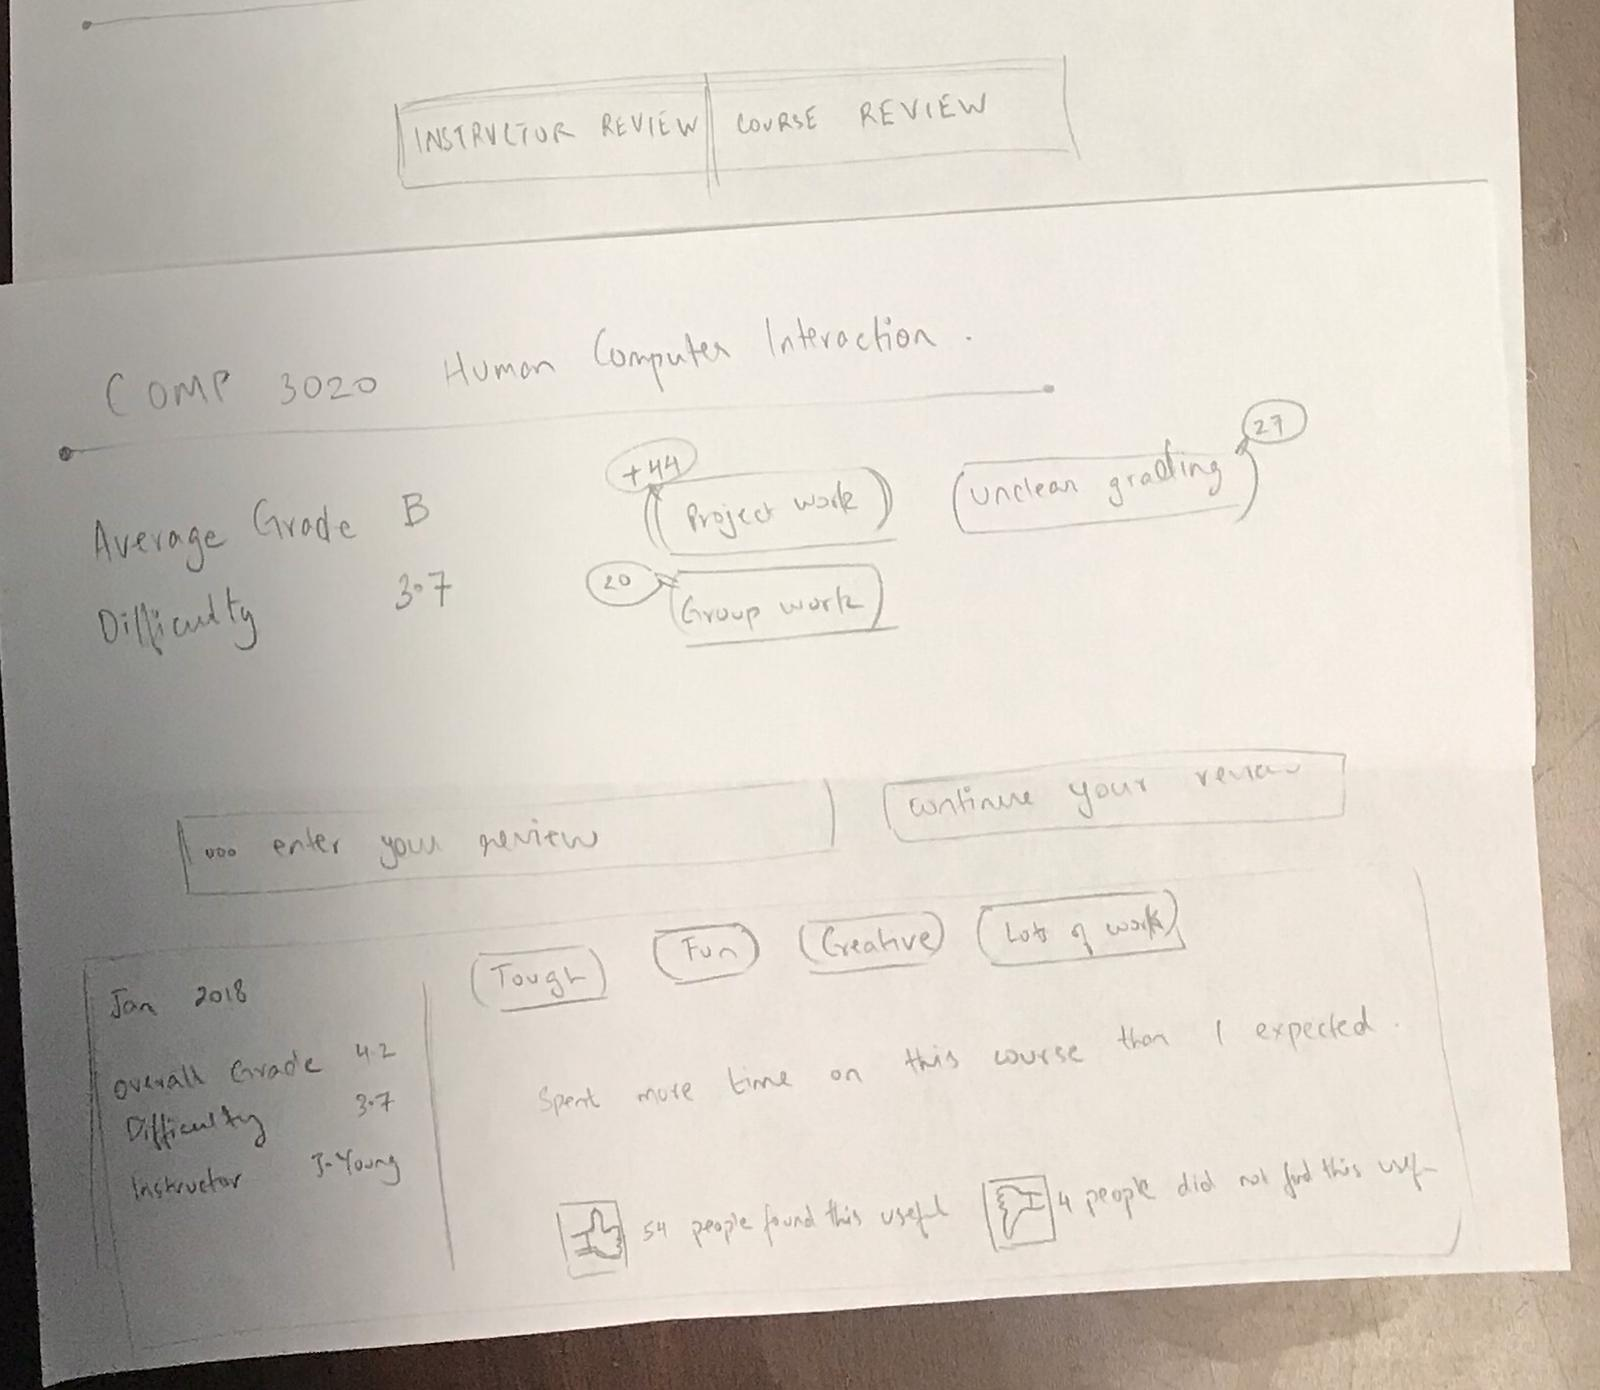
\includegraphics[width=10cm]{ViewCourseInfo_Prototype/paper3-1.jpeg}
\end{figure}
\newline
\newline
\noindent
%As seen in figure 7, the main 'add and remove classes' feature is not explored in this prototype. See paper %prototype 1 and 2 for the ideas we are considering for that feature of the app. 
%\newline\newline
\noindent
As seen in figure 6, the user is able to toggle between instructor reviews and course reviews. The interface for this section is heavily inspired by ratemyprofessor since we know from our research that this website is a popular tool to help inform schedule selection decisions. Through this paper prototype, we were able to confirm that this type of information would be valuable in a course scheduling application. 
\newline
\noindnet
The main limitation to this paper prototype was that the interface was non-native to the user and therefore the user is unsure of what to click or drag. 
\subsection{Figma (web tool) Prototype}
Some of the main design questions for the course research feature revolved around toggle buttons, scrolling, and other desktop features. In order to help us design a better native web interface and gain feedback on the operation of its functionality, a higher-fidelity (but still low-fidelity) prototype was created using a web tool called Figma. 

\begin{figure}[h]
\centering
\caption{Model of Figma Prototype}
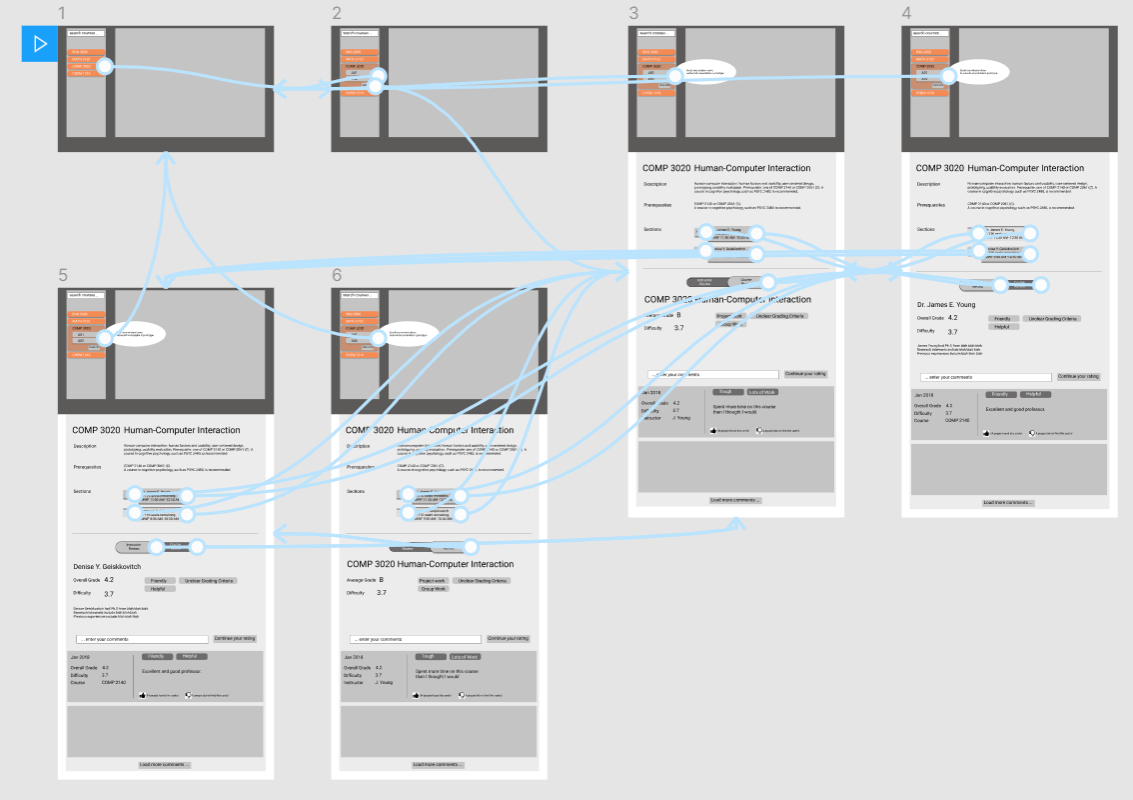
\includegraphics[width=16cm]{ViewCourseInfo_Prototype/uiflow.png}
The diagram in figure 7 was created on Figma by dragging and dropping simple rectangular shapes. The arrows between frames indicate on click events. 
\end{figure}

\vspace{1em}
\noindent
Initially, the screen sits on the main schedule creating feature. That is to say, no detailed course information is displayed.
%\newline
Once the user clicks into a course and selects 'more info', the app auto-scrolls one frame down to display the course information. 
%\newline
A far lighter background theme was used for this section to break similarity with the scheduler frame and indicate to the user that this feature is a pure research tool, and does not directly provide course selection functionality. 
%\newline
In this course and instructor research section, the user was able to toggle between sections and instructors to see standard descriptions and crowd generated reviews.
\newline
\newline
Through this prototype, the goals were to:
\begin{enumerate}[label=\alph*]
\item Discover where the toggle buttons should be and what they should control. Letting users click around and observe their mental model will help inform us of the decisions that need to be made. 
\item Collect feedback on whether students like the reviews and ratings feature and are willing to migrate away from ratemyprofessor to this application. Network effect plays a big role in crowd sourced features such as this one, therefore it is important to find out what will make this application better than ratemyprofessor to attract all the students to this platform instead.
\item Discover what information is crucial to show and what is extraneous. We have some primary user research that has informed this prototype, but this prototype intended to further refine what information students specifically need to make their course selections. 
\end{enumerate}

\section{Informal Prototype Evaluation}
After the prototypes were created, it was important that as much feedback as possible was collected for the designs. Each prototype was presented to multiple research participants who interacted with them, and provided feedback on the designs. This feedback will be relied on to help inform the decisions made when a future prototype is created.


\subsection{Summary of Prototyping Methods}
%includes summary of method for BOTH obtaining feedback, and participants
%~~~~~~~~~~~~~~~~~~~~~~~~~~~~~~~~~~~~~~~~~~~~~~~~~~~~~~~~~~~~~~~~~~~~~~~~~~~~~~~~
%   Both of these paragraphs are initial drafts, written before all feedback was gathered. These MUST be updated and edited between collecting all feedback, and editing the final report. Especially if the other paper prototypes research participants, and feedback methods are not appropriately described by this section -SG
%~~~~~~~~~~~~~~~~~~~~~~~~~~~~~~~~~~~~~~~~~~~~~~~~~~~~~~~~~~~~~~~~~~~~~~~~~~~~~~~~


To obtain feedback for our prototypes, various research participants were asked to participate in evaluating our designs. All participants were university students, and had previously been a part of research for Milestone 1 of this project. The participants provided a wide range of opinions due to various backgrounds within their post secondary studies. The demographic ranged from first year students, to those finishing their degrees. Students in the faculties of science, computer science, and engineering were included. Having such a broad range of participants meant that the feedback represented a large portion of possible users, despite coming from a relatively small number of prototype testers.
\newline 




\subsubsection{Paper Prototyping Methods}
\newline
In testing the paper prototypes, the research participants were presented with an interface. They were not given much instruction so that they could react to the design according to its signifiers and perceived affordances. Using their finger as a cursor, or verbally explaining what they wished to do, the participants navigated the interface and utilized its features. The researcher in each prototype testing session acted as the computer, presenting and arranging various components of the prototypes as necessary. The researcher recorded information about the process taken by the participant, and noted any successes or failures in the design. After given the opportunity to experiment with the prototype, the participant was asked open ended questions about the design. Information regarding what the user thought was good or bad about the design was recorded, as well as suggestions for future iterations. An unrestricted format allowed for gathering feedback regarding many aspects of each design, including features and design elements that may have been overlooked otherwise. This garnered invaluable information to be considered during the next prototyping phase.




\subsubsection{Figma Prototyping Method}
An additional prototype was created on Figma, a prototyping and UI tool that is freely available online. Figma provides an easy drag and drop design interface for shapes, colours, fonts, and not much else. Its prototyping interface allows the designer to link various screens with on-click events, which mimic the feel of a real program. This tool provides a higher fidelity prototype than a paper prototype, but with similar ease. The main benefit to using this was to see the prototype on its native platform and have the user use the same tools (i.e, a mouse's click, hover, and scroll tools) to experiment in the prototype with. 
\newline
\newline
The user was merely given context for the app, and the task they were to perform - which was to chose between section A01 and A02 for the COMP 3020 course. There is absolutely no distinguishing features in terms of reviews and ratings, so the goal was to let them click around and observe what they did instinctively to look for the information that they deemed as important to make this decision. 




\subsection{Summary of Low Fidelity Prototype Feedback}
The feedback for each of the prototypes will guide the continued development of our project. After testing out some ideas that our group decided were potential designs for the final product, we are able to make informed decisions about how to incorporate, change, or exclude each element.
\newline
\newline
From our first prototype we found that users easily understood that contained boxes with the drag icons we used could be dragged and dropped. They also intuitively understood how to use a priority ranking system to generate possible schedules, and still have control over minute details of the scheduling. The visual feedback from the system made sense, the layout of the page worked well, and the meanings of the symbols used were clear. Despite not including the "grey-out" feature suggested during brainstorming, one research participant stated that they would like to be able to use a similar feature. All participants viewed the "black-out" feature as a useful addition, and felt that the priority ranking system was both easy to use, and gave enough control over their scheduling. It was not immediately clear to the users that individual class sections could be moved from the details section to the main priority column, but it was regarded as an important feature. This will be addressed if a similar feature is included in future designs. One participant stated that they would be hesitant to use the trash icon to remove classes unless it was easy to retrieve deleted classes later on. Overall, the interface was successful in being understandable and learnable, and the feedback gained will be useful even if a design based on this prototype is not pursued.
\newline
\newline
Two participants were utilized for the second prototype. Both participants generally agreed that its user interface is definitely better than Aurora's current user interface, but they differed to the degree in which they thought it was better. The first participant definitely found the work-space pane to be a useful feature during the scheduling process. However, the second participant found the work-space pane to be unnecessary as all courses that the user is considering can simply be added to the time-table directly. The second participant then suggested that course conflicts can be visually indicated by overlapping conflicting courses with each other in the time table. Both participants did not find the cost pane useful, as they did not concern themselves with the total cost of courses until the very end of planning. However, both saw that the cost-pane may be useful for working students or students that did not have parents to support them during their education, unlike themselves.
\newline
\newline
The third paper prototype also yielded valuable feedback. When presented to the research participant, it was immediately understood, and the participant remarked at how useful the information and the format it was presented in was. It seemed that displaying the information below the main screen on the same page was a feasible option, rather than having a separate page to navigate to. A toggle to switch between class and professor feedback seemed to work, but it was hard to tell if it would be recognizable or not on a digital interface compared to a paper one. A suggestion was made to clearly differentiate online classes from the rest. This was a valuable consideration, which had not been mentioned by any other research participants, but the merit is easily seen. Some suggestions were given by the research participant, but understanding the feedback from the other interfaces will also contribute to how to successfully incorporate such a feature.
\newline
\newline
The feedback from the Figma prototype was largely positive. Participants had to be reminded that this prototype contained only one feature, as they wanted to continue to experiment with the interface after the intended research was completed. We believe the interactive nature of this web prototype encourages the user to click and explore and this was why the participants tried playing with features that weren't developed yet. With the course description and reviews feature, the participants successfully navigated the different buttons and selections. The interface was similar enough to ratemyprofessor that the participants had no doubt as to how to use it. At the same time, it was distinct enough that the participants understood that this wasn't a direct feed from ratemyprofessor, but a new feature built into this app. There were comments regarding the size of the text, which can and will be remedied in future iterations.


\section{Conclusion}
Throughout the process of Milestone 2 our group learned a lot about how to proceed with our project. Coming up with as many ideas as we did during the brainstorming session greatly pushed our understanding of what was needed to meet our requirements, and introduced many new ideas that would not have otherwise been considered. Focusing on these ideas in depth for the idea polishing and hierarchical task graphs allowed for a more robust view of how to potentially include those ideas in a design. Once our group created the low-fidelity prototypes, it became even clearer what ideas and layouts could work, and gave more insight into what restrictions may come into play later on. Finally, being able to test our ideas with research participants and gain honest feedback on them provided information which will be heavily considered when continuing the design process. knowing what elements are easy to understand and use, and what is unnecessary will help create a learnable, and uncluttered design. Knowing what features are useful, unneeded, and desired will guide the focus on how to meet the requirements defined in Milestone 1. Moving forward, out group is confident in our ability to create a successful design, taking from what was learned throughout this Milestone, and applying it to the next iteration of our design.






%~~~~~~~~~~~~~~~~~~~~~~~~~~~~~~~~~~~~~~~~~~
%   TODO: fix the Appendix title pages so that they look pretty/match the style of the main title pages
%
%   TODO: fix Appendix lettering to match what will happen in the binder
%~~~~~~~~~~~~~~~~~~~~~~~~~~~~~~~~~~~~~~~~~~


%~~~~~~~~~~~~~~~~~~ Appendix Title Pages ~~~~~~~~~~~~

\newpage
\pagenumbering{gobble} %Stop page numbering for Appendix title pages
\vspace*{40mm}
\addcontentsline{toc}{section}{Appendix D: Brainstorming Sketches}
\begin{centering}
	{\huge\bfseries Appendix D: Brainstorming Sketches}\\[0.4cm] 
\end{centering}

%~~~~~~~~~~~~~~~~~~~~~~~~~~~~~~~~~~~~~~~~~~~~~

\newpage	
\vspace*{40mm}
\addcontentsline{toc}{section}{Appendix E: Low - Fidelity Prototypes}
\begin{centering}
	{\huge\bfseries Appendix E: Low - Fidelity Prototypes}\\[0.4cm] 
\end{centering}

%~~~~~~~~~~~~~~~~~~~~~~~~~~~~~~~~~~~~~~~~~~~~~~~

%\newpage	

%\addcontentsline{toc}{section}{Appendix E: Paper Prototype 2}

%	{\huge\bfseries Appendix E: Paper Prototype 2}\\[0.4cm] 

%~~~~~~~~~~~~~~~~~~~~~~~~~~~~~~~~~~~~~~~~~~~~~~~

\newpage	
\vspace*{40mm}
\addcontentsline{toc}{section}{Appendix F: Raw Prototype Feedback}
\begin{centering}
	{\huge\bfseries Appendix F: Raw Prototype Feedback}\\[0.4cm] 
\end{centering}

\newpage

    

    \begin{figure}[h]
        \centering
        Initial state of Figma Prototype
        
        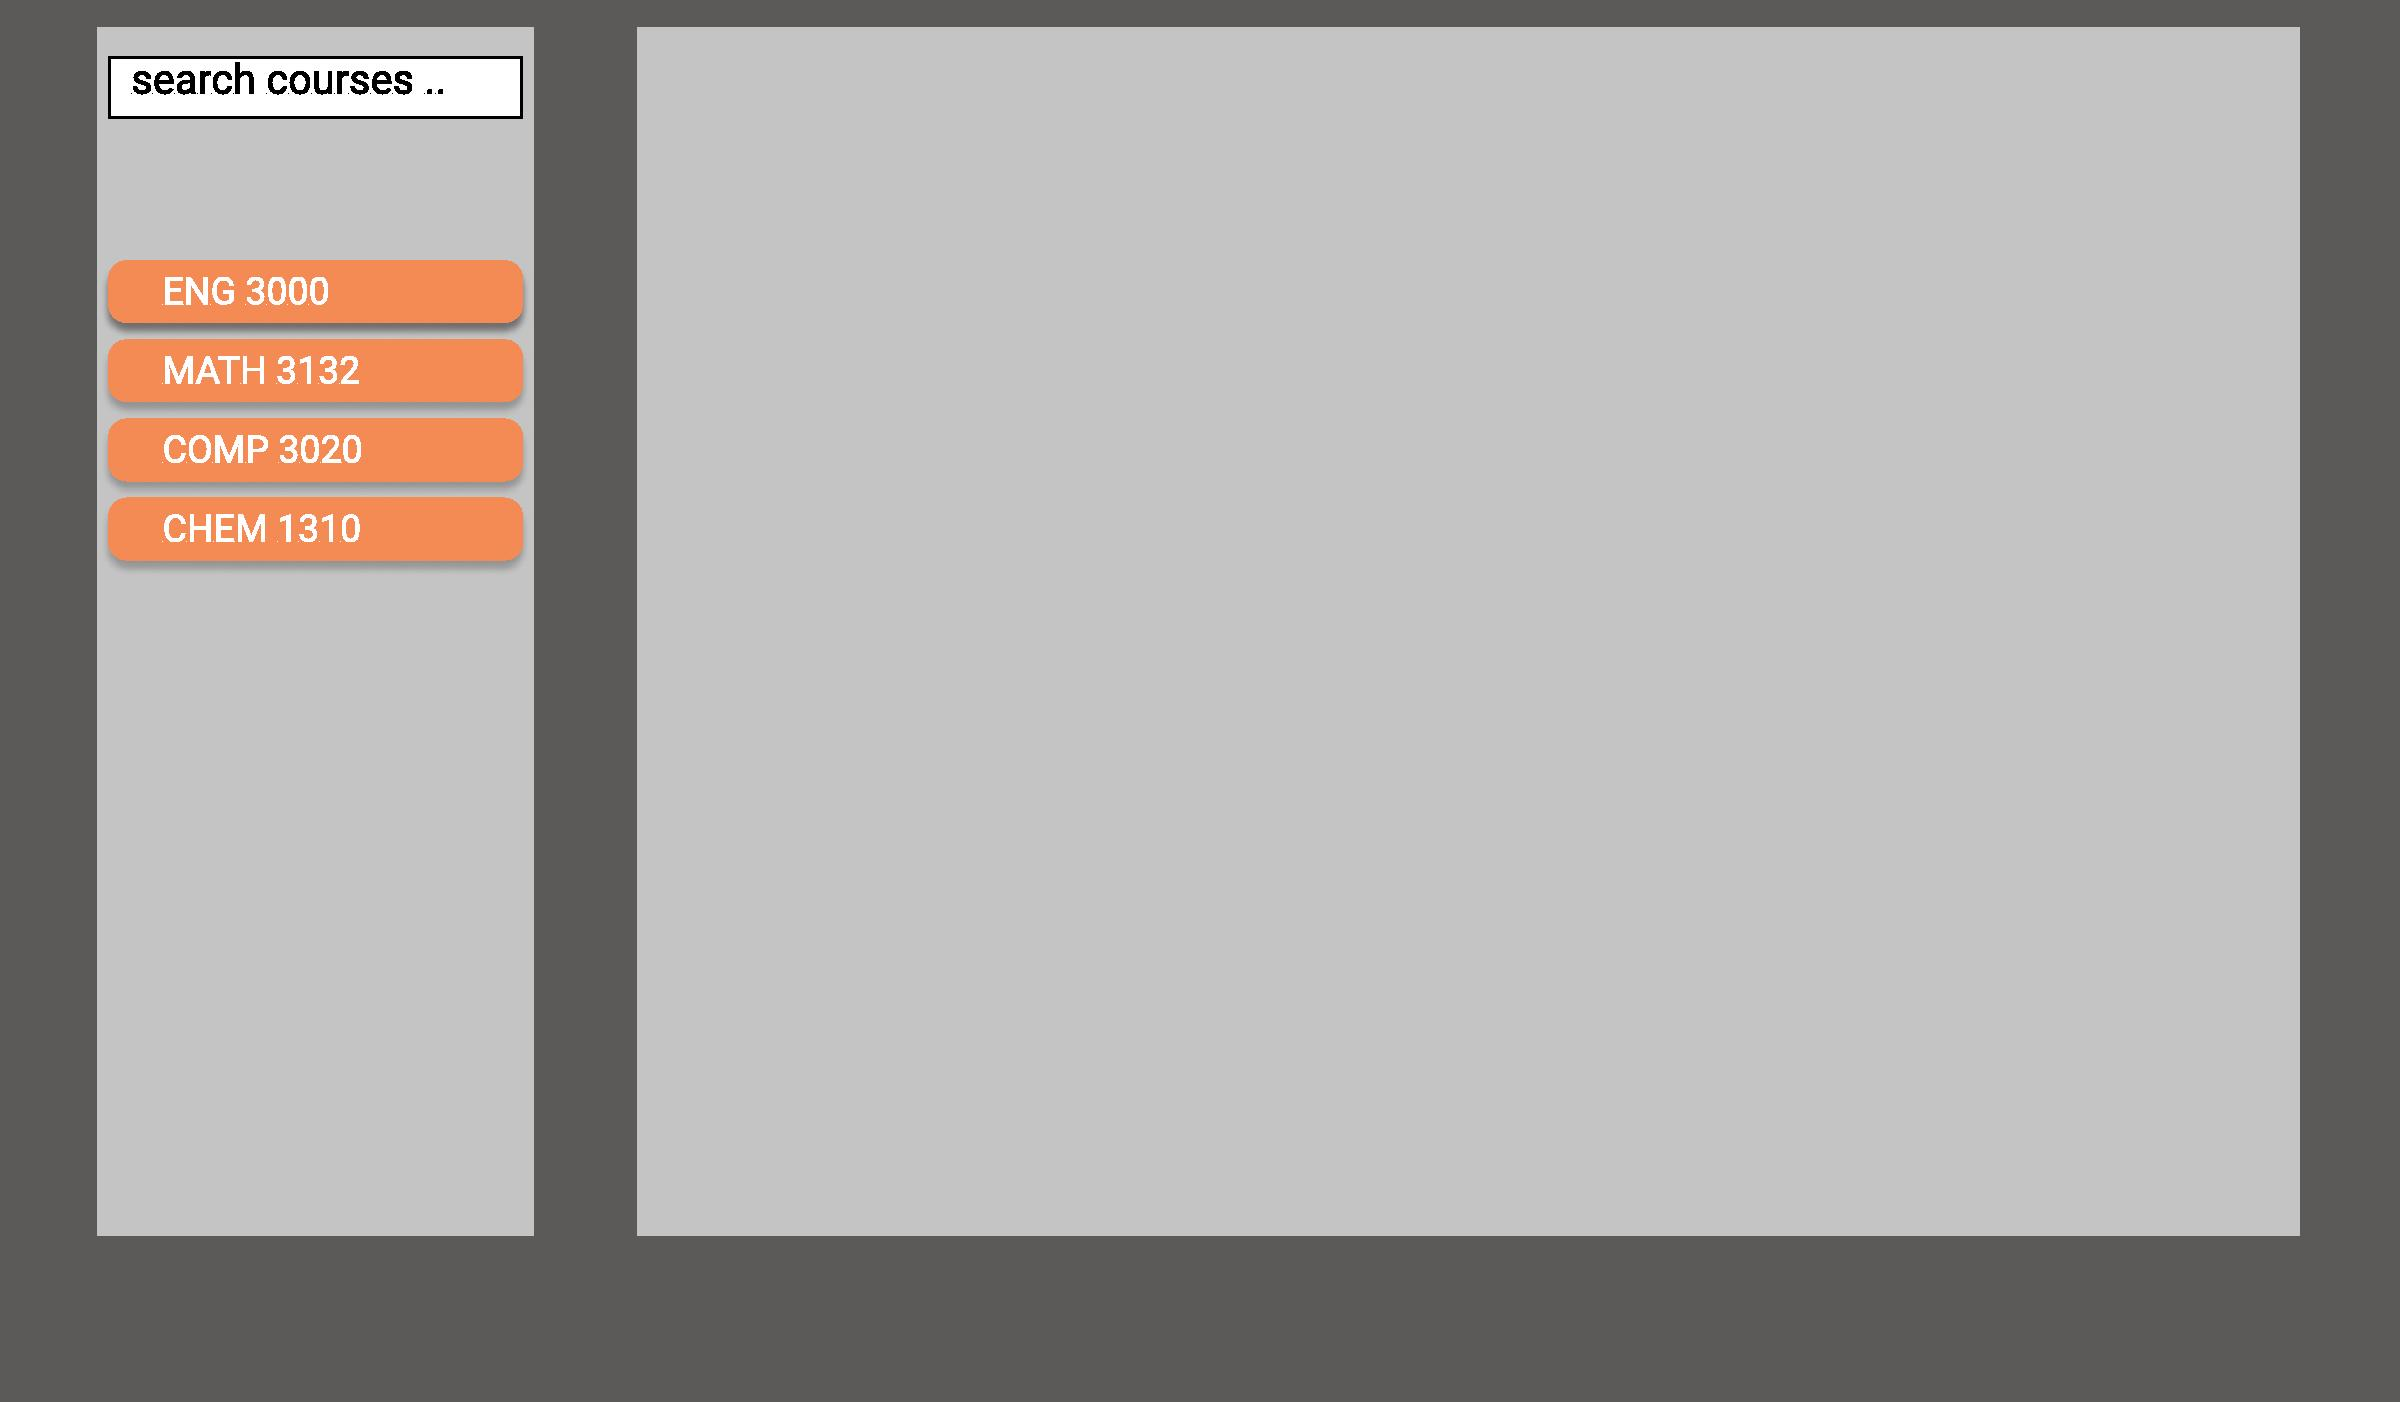
\includegraphics[width=12cm]{ViewCourseInfo_Prototype/Course_Instructor1.jpg}
    \end{figure}
    	
    \vspace{10mm}
    	
    \begin{figure}[h]
        \centering
        Figma Prototype after clicking on "COMP 3020"
        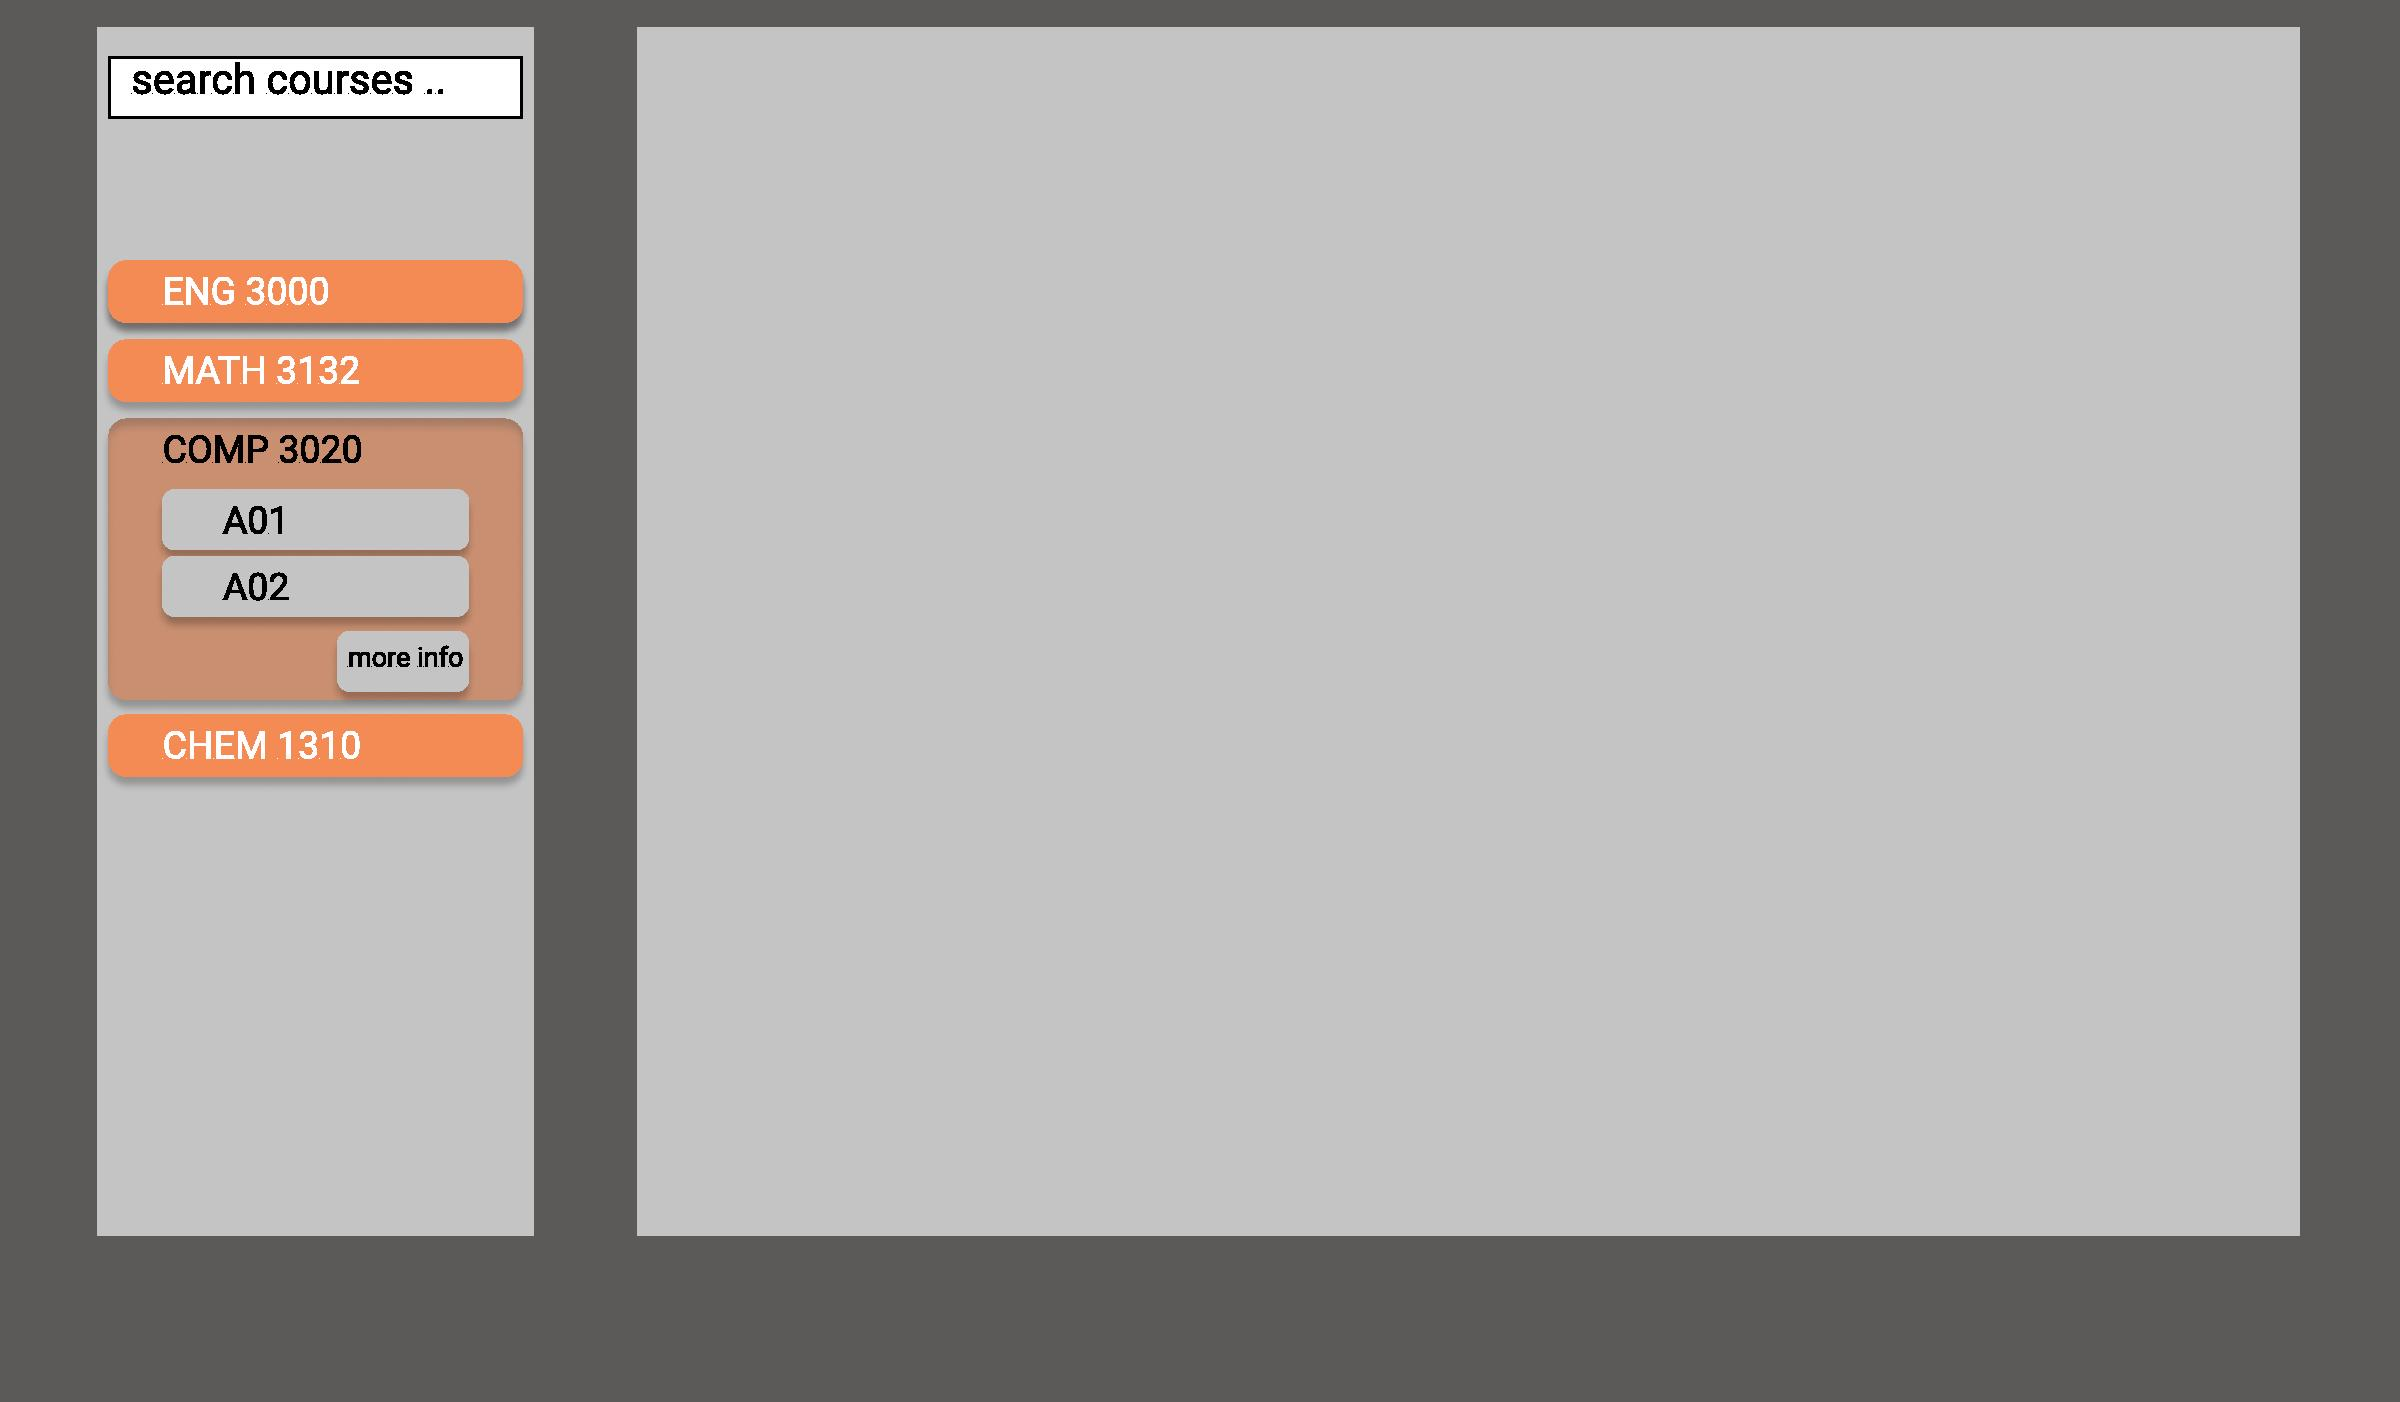
\includegraphics[width=12cm]{ViewCourseInfo_Prototype/Course_Instructor2.jpg}
    \end{figure}
	
\newpage
    \begin{figure}[h]
        \centering
        Figma Prototype showing instructor or course information
        
        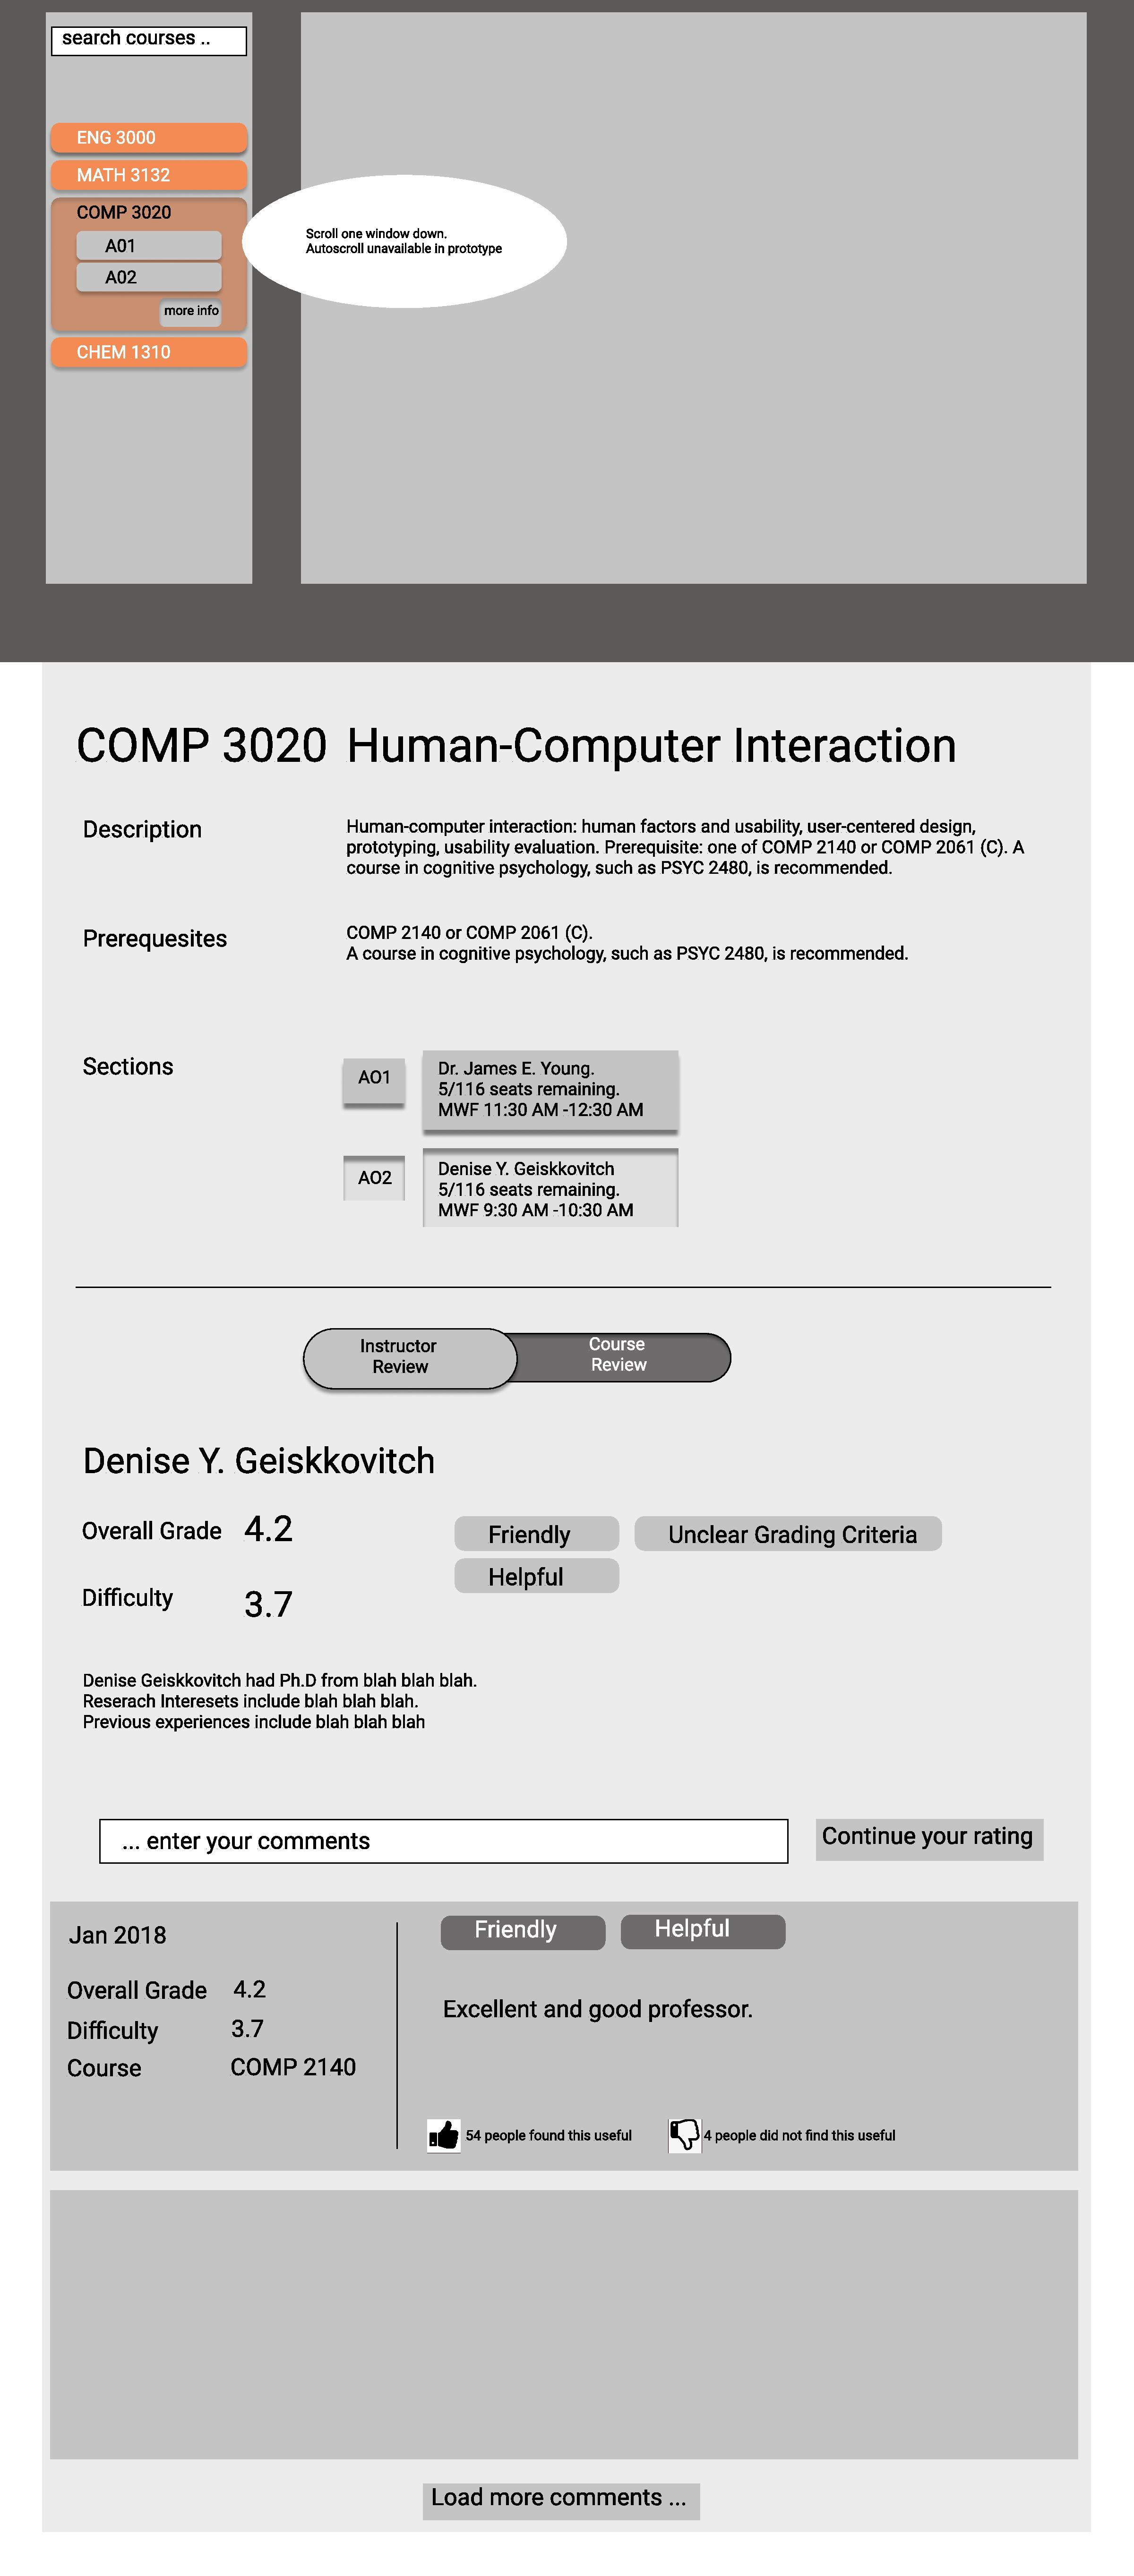
\includegraphics[width=8cm]{ViewCourseInfo_Prototype/Course_Instructor3.jpg}
%    \end{figure}
%\newpage
%    \begin{figure}[h]
%        \centering
%        \caption{Model of Prototype 3}
        \hspace{2mm}
        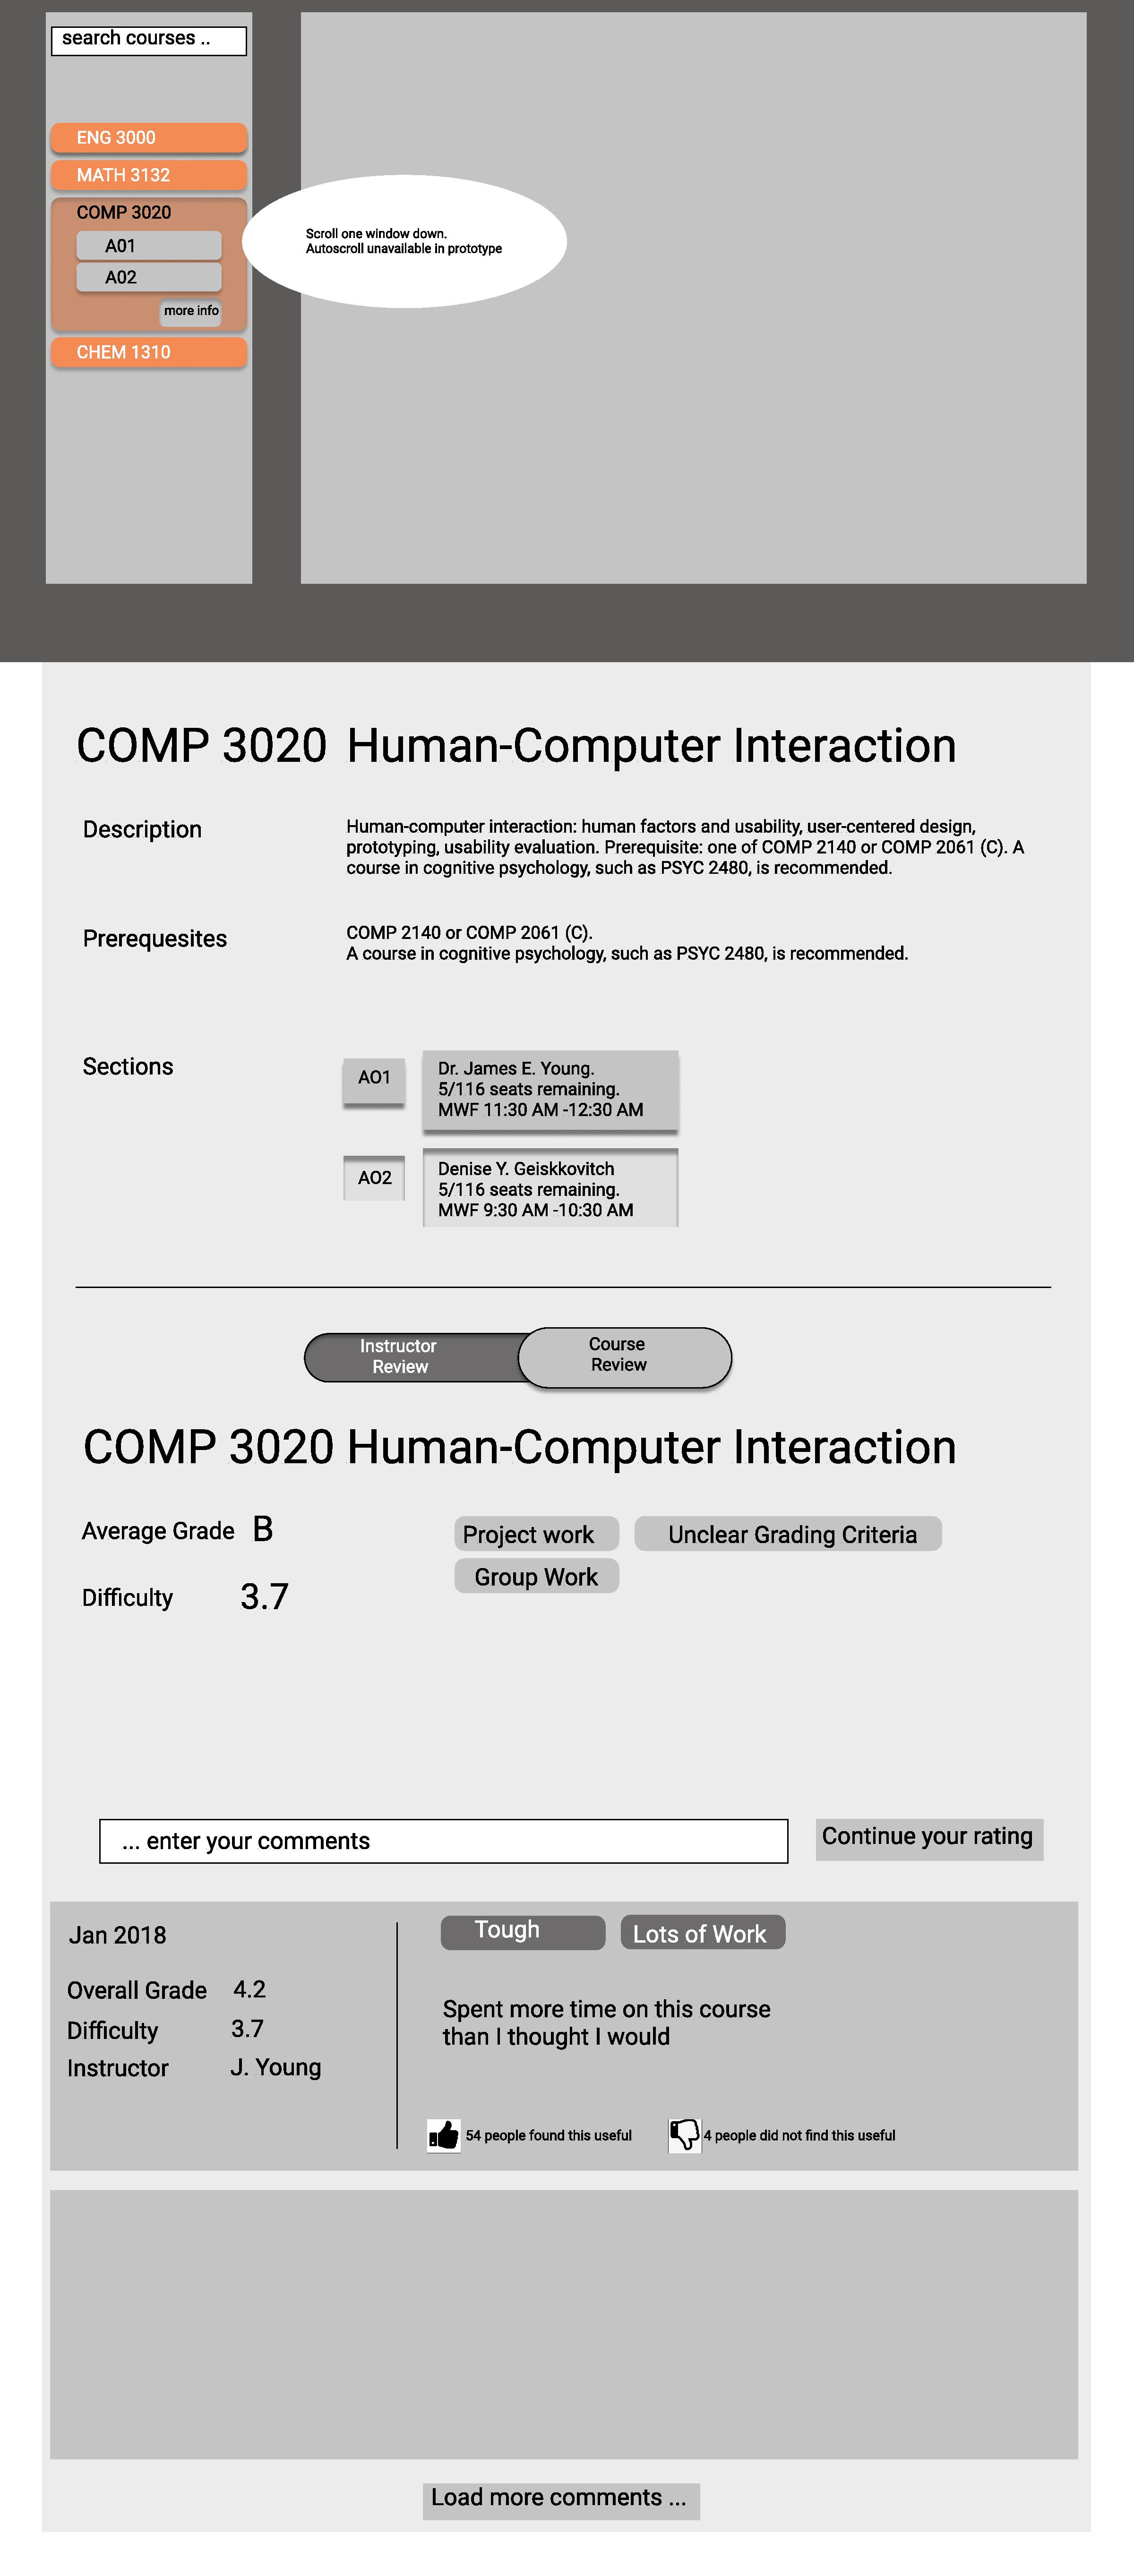
\includegraphics[width=8cm]{ViewCourseInfo_Prototype/Course_Instructor4.jpg}
    \end{figure}
\newpage
    \begin{figure}[h]
        \centering
        %\caption{Figma prototype showing more course and professor information}
        Figma prototype showing more course and professor information

        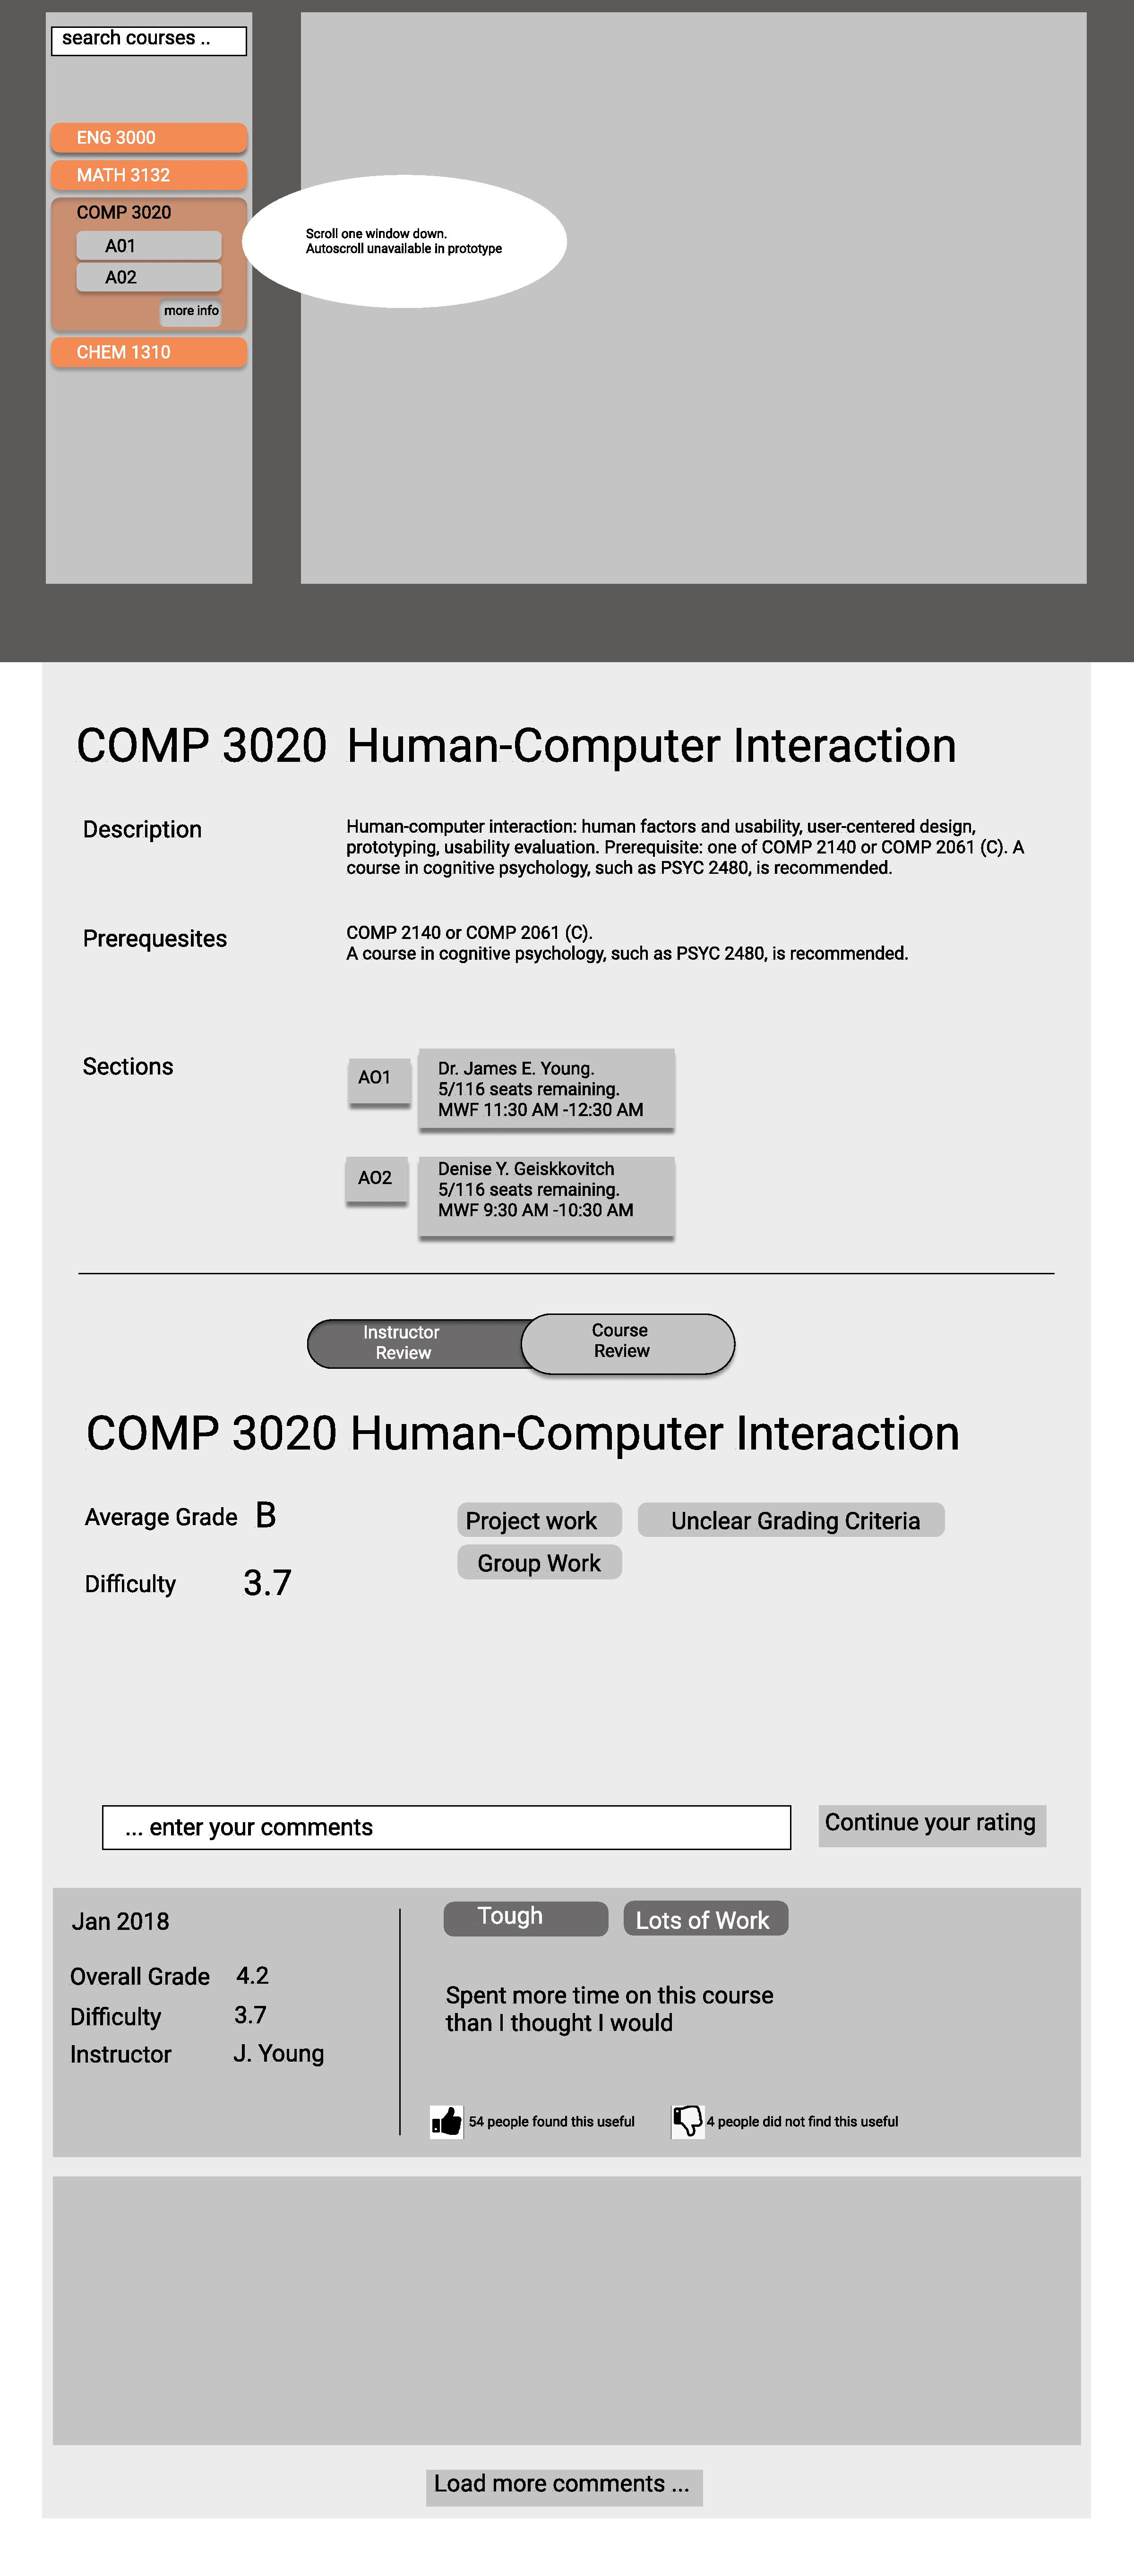
\includegraphics[width=8cm]{ViewCourseInfo_Prototype/Course_Instructor5.jpg}
%    \end{figure}
%\newpage
%    \begin{figure}[h]
%        \centering
%        \caption{Model of Prototype 3}
        \hspace{2mm}
        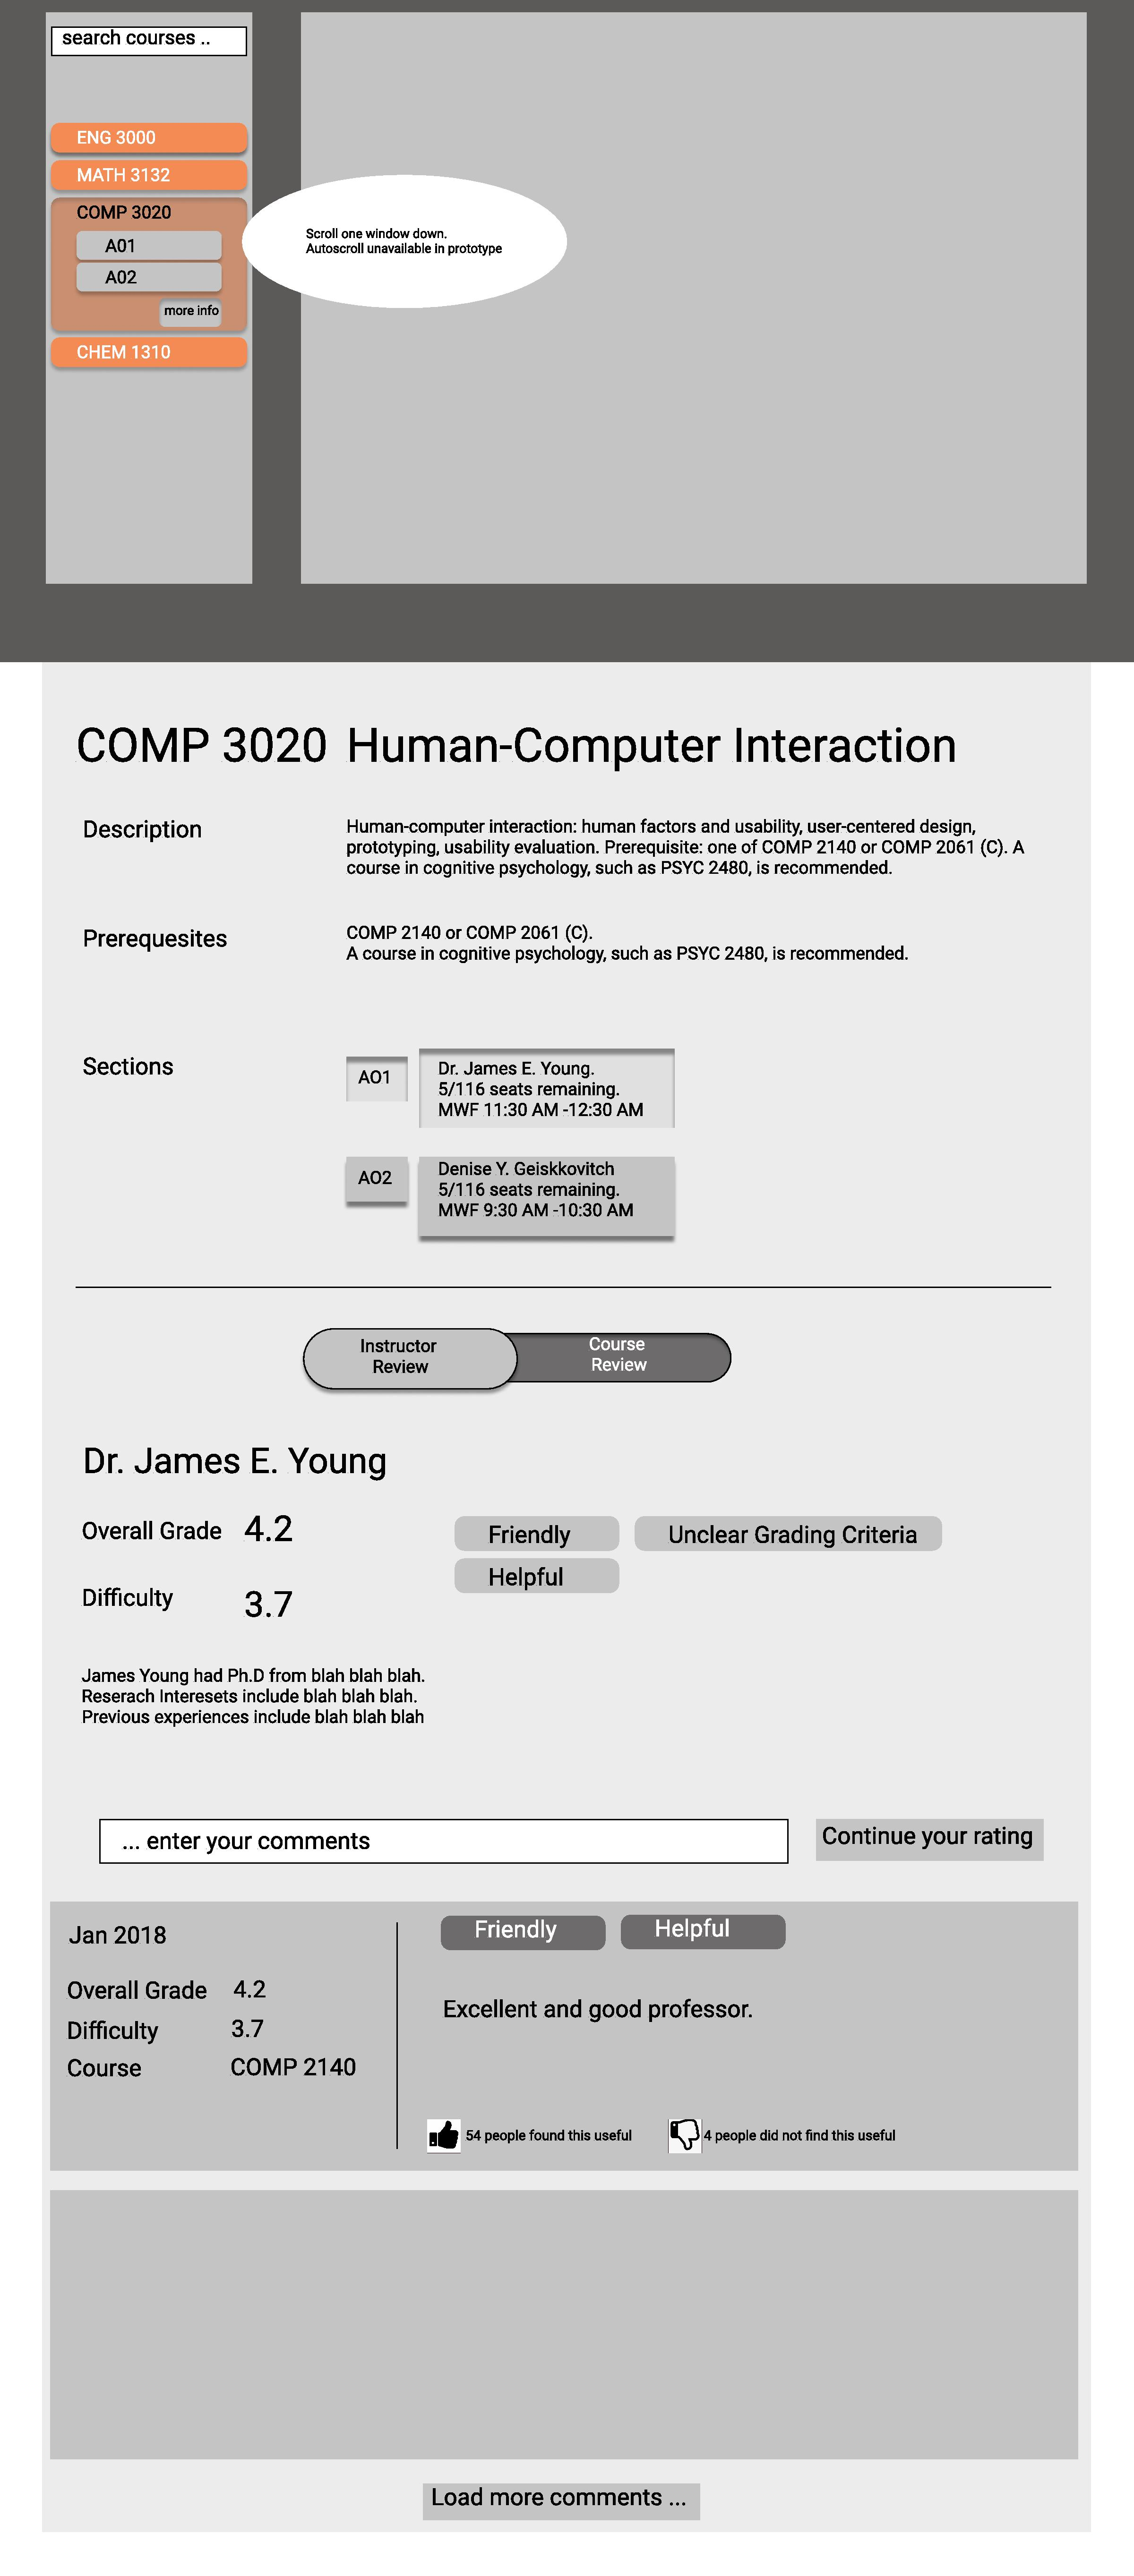
\includegraphics[width=8cm]{ViewCourseInfo_Prototype/Course_Instructor6.jpg}

    \end{figure}



\end{document}
